\documentclass[landscape]{standalone}

\usepackage{tikz}
\usepackage{pgf-umlcd}

\begin{document}

% Lens.h:class PixMapLens : public SampledLens {


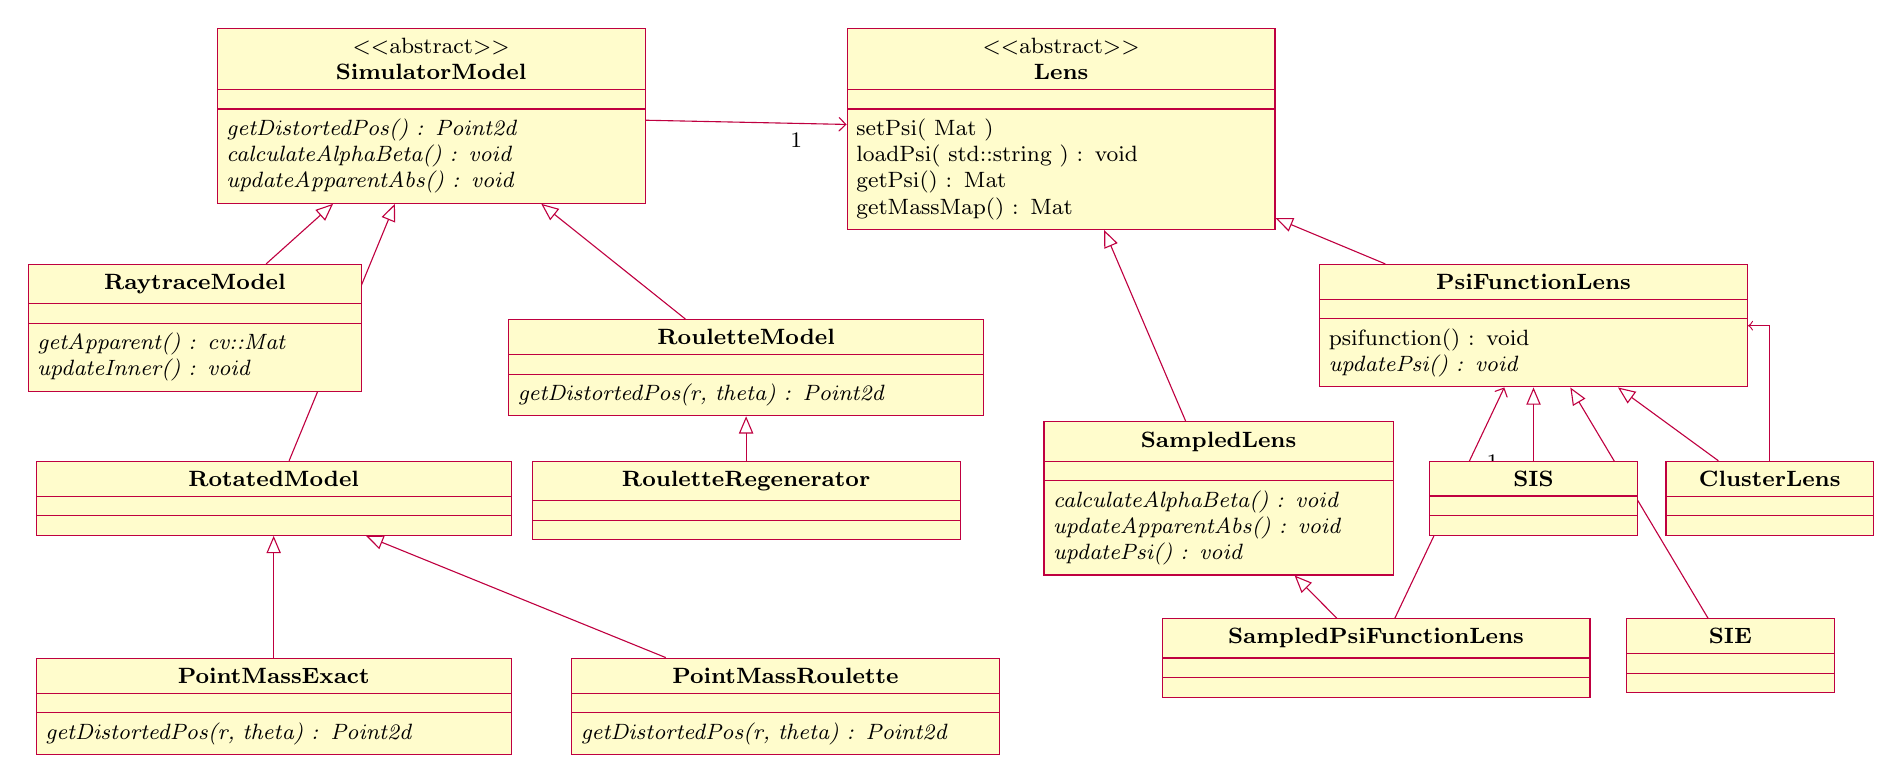
\begin{tikzpicture}
       \tikzstyle{every node}=[font=\footnotesize]

% Simulator.h:class SimulatorModel {
   \begin{abstractclass}[text width = 52mm]{SimulatorModel}{1 , 0}
      \operation[0]{getDistortedPos() : Point2d}
      \operation[0]{calculateAlphaBeta() : void}
      \operation[0]{updateApparentAbs()  : void}
   \end{abstractclass}

% Lens.h:class Lens {
   \begin{abstractclass}[text width = 52mm]{Lens}{9 , 0}
      \operation{setPsi( Mat )}
      \operation{loadPsi( std::string ) : void}
      \operation{getPsi() : Mat}
      \operation{getMassMap() : Mat}
   \end{abstractclass}
   \unidirectionalAssociation{SimulatorModel}{}{1}{Lens}

% Roulette.h:class RouletteModel : public SimulatorModel { 
   \begin{class}[text width = 58mm]{RouletteModel}{5 , -3.7}
      \inherit{SimulatorModel}
      \operation[0]{getDistortedPos(r, theta) : Point2d}
      % \operation[0]{markMask( InputOutputArray )}
      % \operation[0]{maskImage( InputOutputArray )}
      % \operation[0]{getMaskRadius() : double}
   \end{class}


% Simulator.h:class RaytraceModel : public SimulatorModel { 
   \begin{class}[text width = 40mm]{RaytraceModel}{-2 , -3}
      \inherit{SimulatorModel}
      \operation[0]{getApparent() : cv::Mat}
      \operation[0]{updateInner() : void}
   \end{class}

% Simulator.h:class RotatedModel : public SimulatorModel { 
   \begin{class}[text width = 58mm]{RotatedModel}{-1 , -5.5}
      \inherit{SimulatorModel}
   \end{class}

% Simulator.h:class PointMassExact : public RotatedModel { 
   \begin{class}[text width = 58mm]{PointMassExact}{-1 , -8}
      \inherit{RotatedModel}
      \operation[0]{getDistortedPos(r, theta) : Point2d}
   \end{class}

% Simulator.h:class PointMassRoulette : public RotatedModel { 
   \begin{class}[text width = 52mm]{PointMassRoulette}{5.5 , -8}
      \inherit{RotatedModel}
      \operation[0]{getDistortedPos(r, theta) : Point2d}
   \end{class}

% Lens.h:class SampledLens : public Lens {
   \begin{class}[text width = 42mm]{SampledLens}{11 , -5}
      \inherit{Lens}
      \operation[0]{calculateAlphaBeta() : void}
      \operation[0]{updateApparentAbs()  : void}
      \operation[0]{updatePsi()  : void}
   \end{class}

% Lens.h:class PsiFunctionLens : public Lens {
   \begin{class}[text width = 52mm]{PsiFunctionLens}{15 , -3}
      \inherit{Lens}
      \operation{psifunction() : void}
      \operation[0]{updatePsi()  : void}
   \end{class}

% Lens.h:class SampledPsiFunctionLens : public SampledLens {
   \begin{class}[text width = 52mm]{SampledPsiFunctionLens}{13 , -7.5}
      \inherit{SampledLens}
   \end{class}
   \unidirectionalAssociation{SampledPsiFunctionLens}{}{1}{PsiFunctionLens}

% Lens.h:class RouletteLens : public Lens {
   \begin{class}[text width = 52mm]{RouletteRegenerator}{5 , -5.5}
      \inherit{RouletteModel}
   \end{class}

% Lens.h:class SIS : public PsiFunctionLens { 
   \begin{class}[text width = 24mm]{SIS}{15 , -5.5}
      \inherit{PsiFunctionLens}
   \end{class}
   \begin{class}[text width = 24mm]{SIE}{17.5 , -7.5}
      \inherit{PsiFunctionLens}
   \end{class}

% Lens.h:class ClusterLens : public PsiFunctionLens { 
   \begin{class}[text width = 24mm]{ClusterLens}{18 , -5.5}
      \inherit{PsiFunctionLens}
   \end{class}
   % \unidirectionalAssociation{ClusterLens}{}{1..*}{PsiFunctionLens}
   \draw [objectline, ->] 
       (ClusterLens.north) |- (PsiFunctionLens.east) ;

\end{tikzpicture}

\end{document}
